\documentclass[conference]{IEEEtran}
\IEEEoverridecommandlockouts

\usepackage[T1]{fontenc}
\usepackage[utf8]{inputenc}
\usepackage{amsmath,amssymb,amsfonts}
\usepackage{graphicx}
\usepackage{booktabs}
\usepackage{pgfplots}
\usepackage{listings}
\usepackage{xcolor}
\usepackage{cite}
\usepackage{url}
\usepackage{textcomp}
\usepackage{tikz}
\usepackage[hidelinks]{hyperref}

\pgfplotsset{compat=1.18}
\definecolor{serialblue}{HTML}{1F5FD1}
\definecolor{openmpred}{HTML}{D62728}
\definecolor{mpibrown}{HTML}{8C5A2B}
\definecolor{baselinegray}{HTML}{555555}

\lstdefinestyle{cppstyle}{
  language=C++,
  basicstyle=\ttfamily\footnotesize,
  keywordstyle=\color{blue!60!black},
  commentstyle=\color{green!40!black},
  stringstyle=\color{red!55!black},
  numbers=left,
  numberstyle=\tiny\color{gray},
  stepnumber=1,
  numbersep=5pt,
  breaklines=true,
  frame=single,
  columns=fullflexible,
  tabsize=2,
  captionpos=b
}

\title{Pencarian Resep Paralel pada Little Alchemy 2 Menggunakan BFS dan DFS dengan OpenMP dan MPI}

\author{
\makebox[0.96\textwidth][c]{%
\begin{minipage}[t]{0.30\textwidth}
\centering
{\large Muhammad Yusuf Al Azmi\par}
\vspace{0.35em}
{\itshape School of Electrical Engineering and Informatics\par}
{\itshape Bandung Institute of Technology\par}
Bandung, Indonesia\par
13222062@mahasiswa.itb.ac.id
\end{minipage}\hfill
\begin{minipage}[t]{0.30\textwidth}
\centering
{\large Syaugi Adhia Feriyaldi\par}
\vspace{0.35em}
{\itshape School of Electrical Engineering and Informatics\par}
{\itshape Bandung Institute of Technology\par}
Bandung, Indonesia\par
13222068@mahasiswa.itb.ac.id
\end{minipage}\hfill
\begin{minipage}[t]{0.30\textwidth}
\centering
{\large William Gerald Briandelo\par}
\vspace{0.35em}
{\itshape School of Electrical Engineering and Informatics\par}
{\itshape Bandung Institute of Technology\par}
Bandung, Indonesia\par
13222061@mahasiswa.itb.ac.id
\end{minipage}%
}
}

\begin{document}

\maketitle

\begin{abstract}
Little Alchemy 2 merupakan permainan kombinasi elemen yang dapat dipandang sebagai persoalan pencarian pada graf dependensi. Setiap elemen hasil memiliki satu atau lebih pasangan bahan, sehingga proses mencari resep suatu elemen dapat membentuk pohon pencarian yang bercabang. Makalah ini membahas implementasi pencarian resep Little Alchemy 2 menggunakan tiga pendekatan eksekusi, yaitu serial, OpenMP, dan MPI. Implementasi serial dijadikan baseline, OpenMP digunakan untuk paralelisme shared-memory pada satu proses, sedangkan MPI digunakan untuk membagi task pencarian ke beberapa proses. Eksperimen dilakukan pada target \textit{Brick} dengan algoritma BFS, mode \textit{multiple}, limit 50 resep, trace mode \textit{memo}, dan visual mode \textit{shared}. Hasil menunjukkan bahwa OpenMP 4 worker memberi speedup tertinggi pada eksperimen ini, yaitu 1.072 kali terhadap serial. Sebaliknya, MPI lokal dengan 2 dan 4 proses justru lebih lambat karena overhead komunikasi, serialisasi, dan pembagian task lebih besar daripada beban komputasi yang diparalelkan.
\end{abstract}

\begin{IEEEkeywords}
Little Alchemy 2, graf resep, BFS, DFS, memoization, OpenMP, MPI, speedup, efficiency.
\end{IEEEkeywords}

\section{Pendahuluan}

Little Alchemy 2 adalah permainan edukatif-kasual dari Recloak yang meminta pemain menggabungkan dua item untuk menemukan item baru. Situs resmi hint Little Alchemy 2 juga menekankan bahwa hanya dua item yang dapat dicampur pada satu waktu, dan beberapa item dapat membuka banyak kemungkinan kombinasi baru \cite{littlealchemyhints}. Pola permainan seperti ini membuat relasi antar-elemen cukup alami untuk dimodelkan sebagai graf: sebuah elemen hasil memiliki sisi ke dua elemen bahan yang membentuknya.

Dari sudut pandang komputasi, pencarian resep pada Little Alchemy 2 tidak sekadar mencari satu pasangan bahan langsung. Sebuah bahan dapat berupa elemen turunan yang masih harus dicari resepnya lagi sampai mencapai elemen terminal, seperti \textit{Air}, \textit{Earth}, \textit{Fire}, dan \textit{Water}. Oleh karena itu, hasil akhir pencarian lebih tepat direpresentasikan sebagai pohon resep. Masalah menjadi lebih menarik karena satu elemen dapat memiliki banyak resep, dan kombinasi sub-resep dapat membentuk ruang pencarian yang besar.

Proyek ini mengimplementasikan pencarian resep dalam C++17 dengan tiga mode utama: serial, OpenMP, dan MPI. Mode serial dipakai sebagai acuan kebenaran dan baseline waktu. Mode OpenMP memanfaatkan banyak thread pada satu mesin. Mode MPI memecah pencarian menjadi task yang dikerjakan beberapa rank, sehingga pendekatan ini dapat dikembangkan ke banyak komputer. Selain mesin pencarian, proyek juga menyediakan GUI Python untuk menjalankan target, melakukan benchmark, dan menampilkan visualisasi resep.

Makalah ini bertujuan menjelaskan desain sistem, dasar teori, implementasi paralel, serta analisis performa dari data benchmark yang dihasilkan oleh program. Fokus analisis berada pada perbandingan waktu eksekusi, speedup, dan efisiensi terhadap baseline serial.

\section{Rumusan Masalah dan Tujuan}

Masalah utama yang dibahas adalah bagaimana merepresentasikan dan mencari resep Little Alchemy 2 secara benar, lalu bagaimana performa pencarian berubah saat pekerjaan dibagi menggunakan OpenMP dan MPI. Secara lebih spesifik, pertanyaan yang dijawab adalah sebagai berikut.

\begin{enumerate}
  \item Bagaimana resep Little Alchemy 2 direpresentasikan sebagai graf dan pohon pencarian?
  \item Bagaimana algoritma BFS, memoization, dan deduplikasi digunakan untuk menghasilkan resep yang valid?
  \item Bagaimana OpenMP dan MPI diterapkan pada ruang pencarian yang sama?
  \item Bagaimana speedup dan efisiensi dihitung terhadap baseline serial?
  \item Mengapa mode paralel tertentu dapat lebih cepat atau justru lebih lambat dari serial?
\end{enumerate}

Tujuan akhirnya adalah memperoleh laporan performa yang tidak hanya menampilkan angka, tetapi juga menjelaskan alasan teknis di balik angka tersebut.

\section{Dasar Teori}

\subsection{Graf Resep}

Graf resep dapat dipandang sebagai graf berarah terbalik dari elemen hasil ke bahan pembentuknya. Jika \textit{Brick} dapat dibuat dari \textit{Mud} dan \textit{Fire}, maka sistem menyimpan relasi:

\begin{equation}
\textit{Brick} \rightarrow (\textit{Mud}, \textit{Fire})
\end{equation}

Karena setiap resep menggunakan dua bahan, setiap node non-terminal dalam pohon resep memiliki dua anak. Elemen dasar seperti \textit{Air}, \textit{Earth}, \textit{Fire}, dan \textit{Water} dianggap terminal, sehingga pencarian berhenti pada node tersebut walaupun data input mungkin tetap memiliki entri elemen.

\subsection{BFS dan DFS}

Depth-First Search (DFS) menelusuri satu cabang sedalam mungkin sebelum berpindah ke cabang lain. DFS sederhana dan cocok untuk mendapatkan resep pertama berdasarkan urutan data. Breadth-First Search (BFS) memprioritaskan kedalaman yang lebih pendek. Pada proyek ini, BFS memakai pendekatan lazy frontier: kandidat pohon disimpan dalam frontier, lalu node dengan estimasi kedalaman terbaik diproses lebih dulu. Pendekatan ini membantu menghasilkan resep yang relatif pendek lebih awal.

\subsection{Memoization}

Memoization menyimpan hasil pencarian subproblem agar subpohon yang sama tidak dihitung ulang. Pada graf resep, hal ini penting karena banyak elemen muncul sebagai bahan di beberapa resep berbeda. Jika sub-resep \textit{Mud} sudah ditemukan, kemunculan \textit{Mud} berikutnya dapat memakai cache. Pada eksperimen target \textit{Brick} limit 50, cache hit bernilai 0 karena bentuk ekspansi yang diambil tidak menghasilkan reuse cache pada jalur tersebut, tetapi mekanisme ini tetap tersedia untuk target lain yang lebih kompleks.

\subsection{OpenMP}

OpenMP adalah API untuk pemrograman paralel shared-memory di C, C++, dan Fortran \cite{openmp}. Dalam model ini, beberapa thread berjalan dalam satu proses dan berbagi memori yang sama. Biaya komunikasi biasanya lebih kecil dibanding MPI karena data tidak perlu dikirim antar proses melalui message passing. Namun, performa tetap dipengaruhi overhead pembuatan thread, sinkronisasi, dan ukuran pekerjaan yang dibagi.

\subsection{MPI}

Message Passing Interface (MPI) adalah standar untuk pemrograman paralel berbasis pertukaran pesan antar proses \cite{mpiforum}. MPI cocok untuk distributed-memory dan multi-komputer karena setiap proses dapat berjalan pada host berbeda. Standar MPI mencakup komunikasi point-to-point, collective communication, communicator, process topology, dan fitur lain \cite{mpistandard}. Dalam proyek ini, MPI digunakan dengan pola master-worker: rank 0 membagikan task, worker meminta task, menghitung subpohon, lalu mengirim hasil kembali ke master.

\subsection{Speedup dan Efisiensi}

Speedup mengukur seberapa cepat eksekusi paralel dibandingkan baseline serial:

\begin{equation}
S_p = \frac{T_s}{T_p}
\end{equation}

dengan \(T_s\) sebagai waktu serial dan \(T_p\) sebagai waktu eksekusi menggunakan \(p\) worker. Jika \(S_p > 1\), program paralel lebih cepat daripada serial. Jika \(S_p < 1\), program paralel lebih lambat.

Efisiensi mengukur efektivitas rata-rata kontribusi setiap worker:

\begin{equation}
E_p = \frac{S_p}{p}
\end{equation}

Nilai efisiensi ideal adalah 1. Nilai ini berarti setiap worker memberi kontribusi penuh secara linear. Pada praktiknya, efisiensi sering turun karena ada bagian program yang tetap serial, overhead komunikasi, sinkronisasi, startup process, serialisasi data, load imbalance, dan pekerjaan tambahan untuk membagi task.

\section{Desain Sistem}

Sistem terdiri atas beberapa komponen utama. Komponen \textit{common} menyimpan struktur data graf resep, parser JSON, mesin pencarian, statistik, dan visualizer. Tiga executable utama dibangun di atas komponen tersebut: \texttt{alchemy\_serial}, \texttt{alchemy\_openmp}, dan \texttt{alchemy\_mpi}. GUI Python hanya berperan sebagai wrapper untuk memudahkan pemilihan engine, target, parameter, benchmark, dan visualisasi.

Data resep berasal dari \texttt{data/recipes.json}. Dataset lokal berisi 720 elemen dan katalog tier pada \texttt{data/tiers.json} juga memuat 720 elemen. Katalog tier digunakan untuk validasi elemen dan penandaan terminal, termasuk elemen starter dan special.

Gambar hasil resep dibuat oleh visualizer dalam format DOT, lalu dirender menggunakan Graphviz menjadi PNG. Gambar pada Gambar \ref{fig:brick} memperlihatkan contoh resep sederhana untuk target \textit{Brick}. Gambar \ref{fig:lightsword} menunjukkan resep yang lebih dalam dengan subtree yang dipakai ulang.

\begin{figure}[!t]
  \centering
  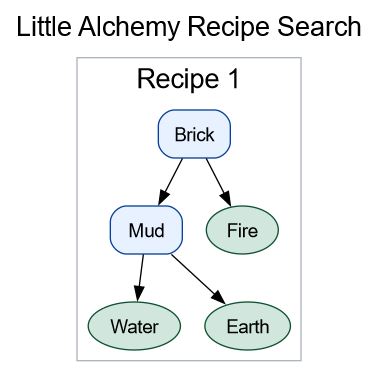
\includegraphics[width=\columnwidth]{gui_run_brick_np6.png}
  \caption{Contoh visualisasi satu resep target \textit{Brick}.}
  \label{fig:brick}
\end{figure}

\begin{figure}[!t]
  \centering
  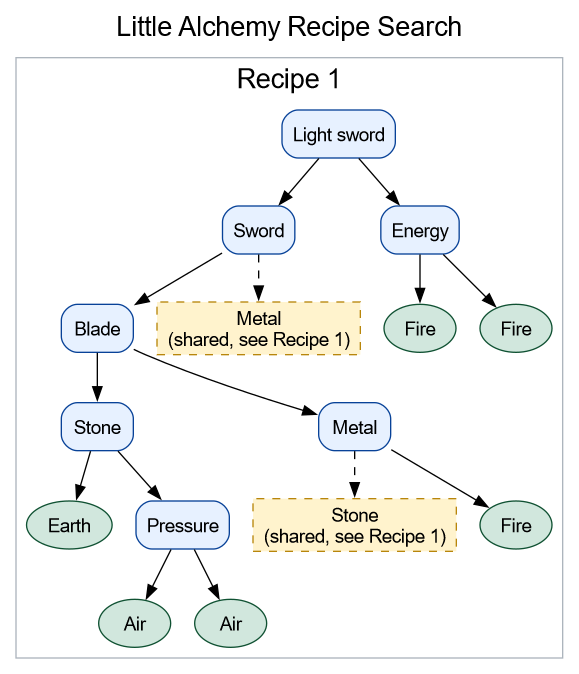
\includegraphics[width=\columnwidth]{light_sword_single.png}
  \caption{Contoh visualisasi resep \textit{Light sword} dengan kedalaman lebih besar dan shared subtree.}
  \label{fig:lightsword}
\end{figure}

\section{Implementasi}

\subsection{Representasi Graf}

Graf resep menyimpan nama elemen secara canonical dan case-insensitive. Pasangan bahan dianggap tidak berurutan, sehingga resep \(A+B\) sama dengan \(B+A\). Elemen dasar langsung ditandai sebagai terminal.

\begin{lstlisting}[style=cppstyle,caption={Inisialisasi elemen dasar pada RecipeGraph.}]
RecipeGraph::RecipeGraph() {
    for (const std::string basic : {"Air", "Earth", "Fire", "Water"}) {
        const auto lower = normalize(basic);
        basicLower_.insert(lower);
        terminalLower_.insert(lower);
        addElement(basic);
    }
}

const std::vector<RecipePair>& RecipeGraph::recipesFor(
        const std::string& name) const {
    const auto canonical = canonicalName(name);
    const auto found = recipesByResult_.find(canonical);
    if (found == recipesByResult_.end() || isTerminal(canonical)) {
        return emptyRecipes_;
    }
    return found->second;
}
\end{lstlisting}

Keputusan menjadikan elemen dasar sebagai terminal membuat pohon resep berhenti pada elemen yang memang tersedia sejak awal permainan. Hal ini sesuai dengan model permainan Little Alchemy 2, yaitu pemain memulai eksplorasi dari elemen dasar.

\subsection{Alur Pencarian}

Kelas \texttt{SearchEngine} menjadi pusat pencarian. Fungsi \texttt{search} melakukan validasi target, reset memo jika diperlukan, menjalankan ekspansi sesuai mode, lalu mengisi statistik waktu, jumlah proses, thread, dan total worker.

\begin{lstlisting}[style=cppstyle,caption={Alur utama pencarian pada SearchEngine.}]
SearchResult SearchEngine::search(const std::string& target,
                                  bool resetMemo) {
    if (!graph_.hasElement(target)) {
        throw std::runtime_error("Target is not available");
    }
    if (resetMemo) {
        clearMemo();
    }
    stats_ = {};

    const auto start = std::chrono::steady_clock::now();
    const auto canonicalTarget = graph_.canonicalName(target);
    auto expanded = options_.mode == SearchMode::All
        ? expandDirectRecipes(canonicalTarget, active)
        : expandElementAny(canonicalTarget,
                           effectiveLimit(options_.limit),
                           active);
    const auto end = std::chrono::steady_clock::now();

    stats_.timeMs =
        std::chrono::duration<double, std::milli>(end - start).count();
    stats_.processes = 1;
    stats_.threadsPerProcess = normalizedThreadCount(options_);
    stats_.totalWorkers = stats_.threadsPerProcess;

    return {canonicalTarget, expanded.trees, stats_};
}
\end{lstlisting}

Pada mode BFS, sistem memakai frontier dan estimasi kedalaman terpendek. Pada mode DFS, sistem mengikuti cabang resep secara rekursif. Deduplikasi dilakukan menggunakan signature pohon agar resep yang sama dengan urutan bahan terbalik tidak dihitung dua kali.

\subsection{Paralelisasi OpenMP}

OpenMP digunakan pada ekspansi BFS lazy. Frontier dengan estimasi yang sama dikumpulkan menjadi batch, lalu batch tersebut diproses paralel. Penjadwalan \texttt{dynamic} dipilih karena biaya ekspansi tiap state tidak selalu sama.

\begin{lstlisting}[style=cppstyle,caption={Ekspansi batch BFS menggunakan OpenMP.}]
std::vector<FrontierExpansion> expansions(batch.size());

#pragma omp parallel for schedule(dynamic) num_threads(threadCount)
for (int i = 0; i < static_cast<int>(batch.size()); ++i) {
    expansions[static_cast<std::size_t>(i)] =
        expandFrontierState(graph_, depthMap,
            std::move(batch[static_cast<std::size_t>(i)]));
}

for (auto& expansion : expansions) {
    stats_.nodesVisited += expansion.nodesVisited;
    for (auto& state : expansion.states) {
        pushState(std::move(state));
    }
}
\end{lstlisting}

Model ini menjaga agar struktur frontier utama tetap dikonsolidasikan di thread utama setelah batch selesai. Dengan begitu, hasil tetap lebih mudah dikendalikan dan dibandingkan terhadap serial.

\subsection{Paralelisasi MPI}

Pada MPI, rank 0 bertindak sebagai master. Master membangun task dari target berdasarkan \texttt{split-depth}, lalu worker meminta task. Setelah worker menyelesaikan partial tree, hasil dikirim kembali sebagai payload JSON. Master menggabungkan hasil, menghapus duplikat, dan membatasi jumlah resep sesuai limit.

\begin{lstlisting}[style=cppstyle,caption={Pola komunikasi master-worker pada MPI.}]
while (activeWorkers > 0) {
    MPI_Status status;
    MPI_Probe(MPI_ANY_SOURCE, MPI_ANY_TAG,
              MPI_COMM_WORLD, &status);

    if (status.MPI_TAG == MPI_TAG_REQUEST) {
        receiveEmptyRequest(status, masterCommSeconds);
        if (nextTask < payloads.size() &&
            !limitReached(recipes.size(), limit)) {
            sendString(status.MPI_SOURCE, MPI_TAG_TASK,
                       payloads[nextTask], masterCommSeconds);
            ++nextTask;
        } else {
            sendString(status.MPI_SOURCE, MPI_TAG_STOP,
                       "", masterCommSeconds);
            --activeWorkers;
        }
    } else if (status.MPI_TAG == MPI_TAG_RESULT) {
        const auto payloadText =
            receiveString(status, masterCommSeconds);
        mergeWorkerResult(nlohmann::json::parse(payloadText),
                          limit, recipes, nullptr, seen, stats);
    }
}
\end{lstlisting}

Pendekatan ini fleksibel untuk multi-komputer, tetapi overhead-nya lebih besar dibanding OpenMP. Setiap hasil harus melewati komunikasi MPI, parsing JSON, dan penggabungan di master. Selain itu, memoization pada MPI bersifat lokal per worker, bukan cache global bersama.

\subsection{Perhitungan Speedup dan Efisiensi}

Perhitungan speedup dan efisiensi dilakukan dari baseline serial. Pada mode compare GUI, baseline diambil dari baris engine serial, kemudian setiap varian dibandingkan terhadap waktu tersebut.

\begin{lstlisting}[style=cppstyle,caption={Rumus speedup dan efficiency pada statistik MPI.}]
if (options.baselineMs > 0.0 && stats.timeMs > 0.0) {
    stats.speedup = options.baselineMs / stats.timeMs;
    stats.efficiency =
        stats.speedup / static_cast<double>(
            std::max(1, stats.totalWorkers));
}
\end{lstlisting}

Walaupun cuplikan tersebut berasal dari jalur MPI, rumus yang sama digunakan pada pembacaan CSV compare untuk serial, OpenMP, dan MPI.

\section{Metodologi Eksperimen}

Eksperimen dilakukan melalui fitur \textit{Run Compare} pada GUI. Semua varian memakai target dan parameter pencarian yang sama agar perbandingan adil. Konfigurasi eksperimen adalah sebagai berikut:

\begin{itemize}
  \item Target: \textit{Brick}.
  \item Algorithm: BFS.
  \item Mode: \textit{multiple}.
  \item Limit: 50 resep.
  \item Trace mode: \textit{memo}.
  \item Visual mode: \textit{shared}.
  \item Render: JSON.
  \item Baseline: waktu serial.
\end{itemize}

Varian yang dibandingkan adalah serial 1 worker, OpenMP 2 thread, OpenMP 4 thread, MPI lokal 2 proses, dan MPI lokal 4 proses. Metrik yang dicatat meliputi waktu total, waktu komunikasi, jumlah resep ditemukan, speedup, dan efisiensi.

\section{Hasil dan Analisis}

\subsection{Hasil Benchmark}

Tabel \ref{tab:benchmark} menampilkan hasil dari file \texttt{results/gui\_run\_compare.csv}. Semua varian berhasil menemukan 50 resep, sehingga perbandingan waktu dapat dianggap membandingkan pekerjaan output yang sama.

\begin{table*}[!t]
\centering
\caption{Hasil benchmark pencarian resep \textit{Brick} limit 50.}
\label{tab:benchmark}
\footnotesize
\begin{tabular}{lrrrrrrr}
\toprule
Varian & Proses & Thread/rank & Worker & Waktu (ms) & Komunikasi (ms) & Speedup & Efisiensi \\
\midrule
Serial & 1 & 1 & 1 & 92.6897 & 0.0000 & 1.000 & 1.000 \\
OpenMP 2 & 1 & 2 & 2 & 88.7091 & 0.0000 & 1.045 & 0.522 \\
OpenMP 4 & 1 & 4 & 4 & 86.4973 & 0.0000 & 1.072 & 0.268 \\
MPI lokal 2 & 2 & 1,1 & 2 & 395.6022 & 332.7728 & 0.234 & 0.117 \\
MPI lokal 4 & 4 & 1,1,1,1 & 4 & 542.2323 & 613.0017 & 0.171 & 0.043 \\
\bottomrule
\end{tabular}
\end{table*}

OpenMP 2 thread menurunkan waktu dari 92.6897 ms menjadi 88.7091 ms. OpenMP 4 thread menurunkan waktu lagi menjadi 86.4973 ms. Peningkatan ini ada, tetapi tidak besar. Artinya, beban pencarian target \textit{Brick} dengan limit 50 belum cukup berat untuk menghasilkan scaling tinggi.

MPI lokal 2 proses membutuhkan 395.6022 ms, sedangkan MPI lokal 4 proses membutuhkan 542.2323 ms. Keduanya lebih lambat daripada serial. Ini menunjukkan bahwa untuk beban kerja ini, biaya komunikasi dan koordinasi MPI lebih dominan daripada penghematan waktu pencarian.

\subsection{Waktu Eksekusi}

Gambar \ref{fig:timeplot} menunjukkan waktu eksekusi terhadap jumlah worker/thread. Titik pada \(x=1\) adalah baseline serial, bukan OpenMP atau MPI satu proses. Karena eksperimen paralel hanya dijalankan pada 2 dan 4 worker, kurva OpenMP dan MPI lokal dimulai dari \(x=2\).

\begin{figure}[!t]
\centering
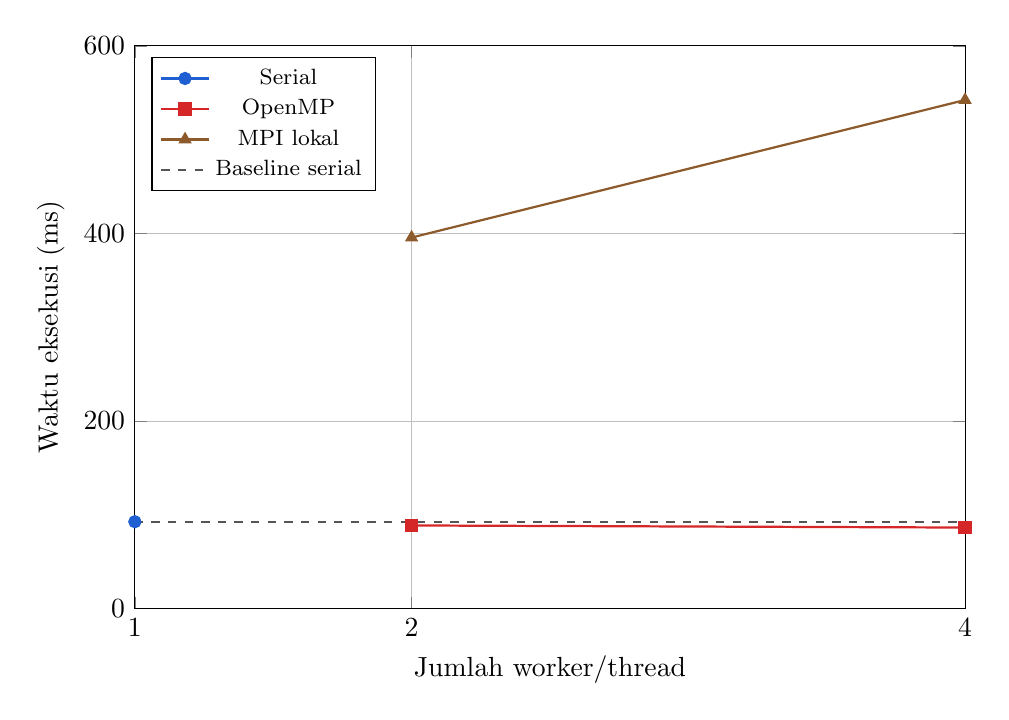
\begin{tikzpicture}
\begin{axis}[
    width=\columnwidth,
    height=0.72\columnwidth,
    xlabel={Jumlah worker/thread},
    ylabel={Waktu eksekusi (ms)},
    xmin=1,
    xmax=4,
    ymin=0,
    ymax=600,
    xtick={1,2,4},
    ytick={0,200,400,600},
    grid=major,
    legend style={
      font=\footnotesize,
      at={(0.02,0.98)},
      anchor=north west,
      draw=black,
      fill=white
    }
]
\addplot+[serialblue, mark=*, thick, mark options={fill=serialblue}] coordinates {(1,92.6897)};
\addlegendentry{Serial}
\addplot+[openmpred, mark=square*, thick, mark options={fill=openmpred}] coordinates {(2,88.7091) (4,86.4973)};
\addlegendentry{OpenMP}
\addplot+[mpibrown, mark=triangle*, thick, mark options={fill=mpibrown}] coordinates {(2,395.6022) (4,542.2323)};
\addlegendentry{MPI lokal}
\addplot+[baselinegray, dashed, thick, mark=none] coordinates {(1,92.6897) (4,92.6897)};
\addlegendentry{Baseline serial}
\end{axis}
\end{tikzpicture}
\caption{Perbandingan waktu eksekusi terhadap jumlah worker/thread.}
\label{fig:timeplot}
\end{figure}

Pada OpenMP, waktu sedikit menurun saat jumlah thread dinaikkan. Hal ini masuk akal karena ekspansi batch BFS dapat dibagi ke beberapa thread, tetapi bagian pengelolaan frontier, deduplikasi, dan penggabungan hasil tetap dilakukan secara terpusat. Selain itu, beban target \textit{Brick} relatif kecil, sehingga overhead thread dan sinkronisasi masih cukup terasa.

Pada MPI, waktu meningkat ketika jumlah proses dinaikkan dari 2 menjadi 4. Hal ini dapat terjadi karena task yang tersedia tidak cukup banyak atau tidak cukup berat untuk mengimbangi overhead komunikasi. Master juga harus melakukan \texttt{MPI\_Probe}, menerima request, mengirim task, menerima payload hasil, melakukan parsing, lalu menggabungkan recipe. Semakin banyak rank, semakin banyak koordinasi yang harus dilakukan.

\subsection{Speedup dan Efisiensi}

Gambar \ref{fig:speedupplot} menampilkan speedup terhadap baseline serial. Plot ini tetap menggunakan sumbu worker karena metrik speedup memang dibaca sebagai fungsi jumlah worker. Baseline \(S=1\) berarti performa sama dengan serial; titik di atas garis tersebut lebih cepat, sedangkan titik di bawahnya lebih lambat.

\begin{figure}[!t]
\centering
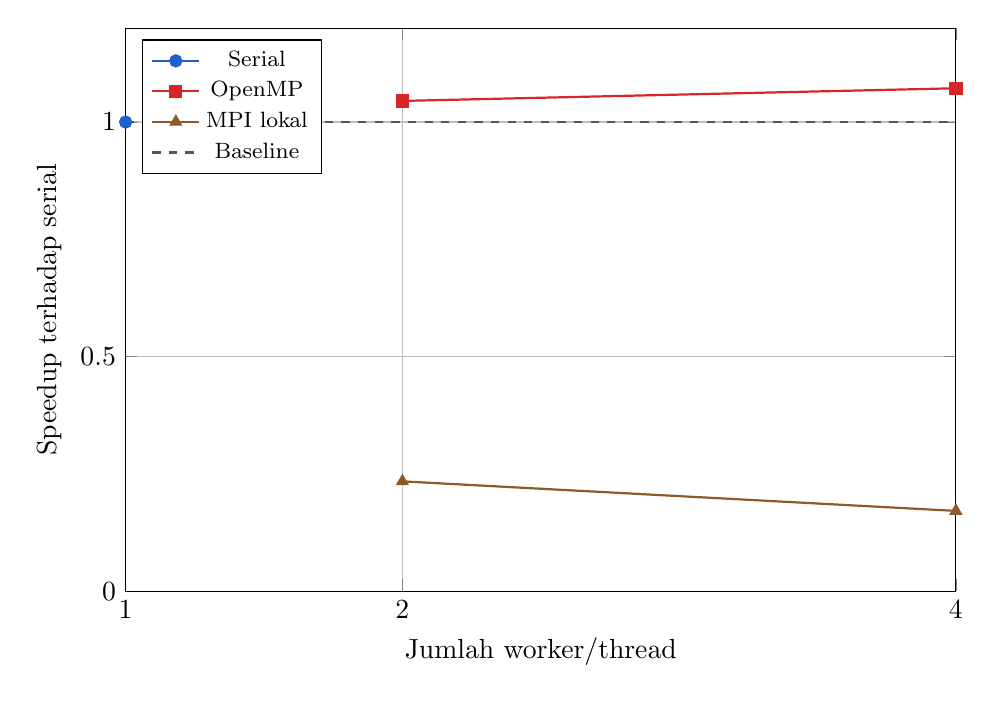
\begin{tikzpicture}
\begin{axis}[
    width=\columnwidth,
    height=0.72\columnwidth,
    xlabel={Jumlah worker/thread},
    ylabel={Speedup terhadap serial},
    xmin=1,
    xmax=4,
    ymin=0,
    ymax=1.2,
    xtick={1,2,4},
    ytick={0,0.5,1.0},
    grid=major,
    legend style={
      font=\footnotesize,
      at={(0.02,0.98)},
      anchor=north west,
      draw=black,
      fill=white
    }
]
\addplot+[serialblue, mark=*, thick, mark options={fill=serialblue}] coordinates {(1,1.000)};
\addlegendentry{Serial}
\addplot+[openmpred, mark=square*, thick, mark options={fill=openmpred}] coordinates {(2,1.045) (4,1.072)};
\addlegendentry{OpenMP}
\addplot+[mpibrown, mark=triangle*, thick, mark options={fill=mpibrown}] coordinates {(2,0.234) (4,0.171)};
\addlegendentry{MPI lokal}
\addplot+[baselinegray, dashed, thick, mark=none] coordinates {(1,1.000) (4,1.000)};
\addlegendentry{Baseline}
\end{axis}
\end{tikzpicture}
\caption{Speedup OpenMP dan MPI lokal terhadap baseline serial.}
\label{fig:speedupplot}
\end{figure}

Gambar \ref{fig:efficiencyplot} memperlihatkan efisiensi paralel. Sama seperti plot sebelumnya, titik \(x=1\) hanya merepresentasikan serial sebagai baseline ideal.

\begin{figure}[!t]
\centering
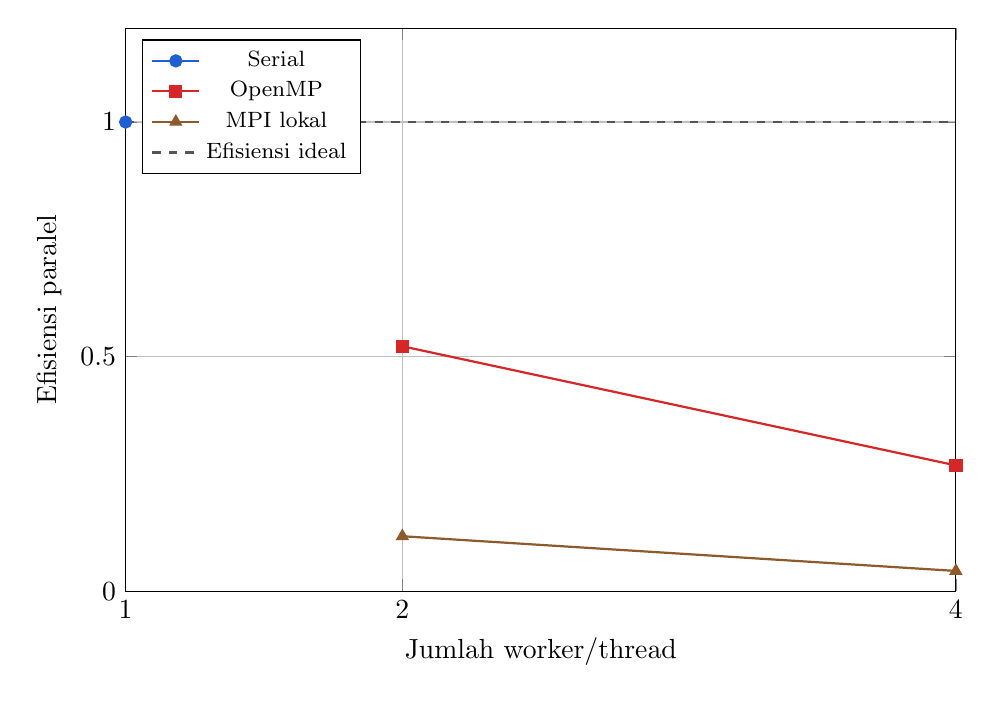
\begin{tikzpicture}
\begin{axis}[
    width=\columnwidth,
    height=0.72\columnwidth,
    xlabel={Jumlah worker/thread},
    ylabel={Efisiensi paralel},
    xmin=1,
    xmax=4,
    ymin=0,
    ymax=1.2,
    xtick={1,2,4},
    ytick={0,0.5,1.0},
    grid=major,
    legend style={
      font=\footnotesize,
      at={(0.02,0.98)},
      anchor=north west,
      draw=black,
      fill=white
    }
]
\addplot+[serialblue, mark=*, thick, mark options={fill=serialblue}] coordinates {(1,1.000)};
\addlegendentry{Serial}
\addplot+[openmpred, mark=square*, thick, mark options={fill=openmpred}] coordinates {(2,0.522) (4,0.268)};
\addlegendentry{OpenMP}
\addplot+[mpibrown, mark=triangle*, thick, mark options={fill=mpibrown}] coordinates {(2,0.117) (4,0.043)};
\addlegendentry{MPI lokal}
\addplot+[baselinegray, dashed, thick, mark=none] coordinates {(1,1.000) (4,1.000)};
\addlegendentry{Efisiensi ideal}
\end{axis}
\end{tikzpicture}
\caption{Efisiensi paralel OpenMP dan MPI lokal terhadap jumlah worker/thread.}
\label{fig:efficiencyplot}
\end{figure}

Efisiensi OpenMP 2 adalah 0.522. Artinya, dua thread secara rata-rata hanya menghasilkan 52.2\% dari kontribusi ideal per thread. OpenMP 4 memiliki efisiensi 0.268, yang berarti penambahan thread masih mempercepat waktu total, tetapi kontribusi tambahan per thread makin kecil. Ini adalah gejala umum pada workload kecil: bagian paralel tidak cukup besar untuk menutupi overhead dan bagian serial.

Efisiensi MPI lokal jauh lebih rendah, yaitu 0.117 untuk 2 proses dan 0.043 untuk 4 proses. Karena speedup MPI sudah di bawah 1, efisiensi juga otomatis rendah. Dalam konteks ini, rendahnya efisiensi bukan berarti hasil MPI salah, tetapi menunjukkan bahwa konfigurasi eksperimen tidak cocok untuk MPI lokal. MPI lebih masuk akal untuk workload yang jauh lebih berat, task yang lebih banyak, atau skenario multi-komputer yang memang membutuhkan distributed-memory.

\subsection{Analisis Waktu Komunikasi MPI}

Gambar \ref{fig:commplot} menampilkan communication time dari setiap varian. Serial dan OpenMP berada pada 0 ms karena tidak melakukan komunikasi antar-rank MPI, sedangkan MPI lokal memiliki biaya komunikasi yang terlihat dominan.

\begin{figure}[!t]
\centering
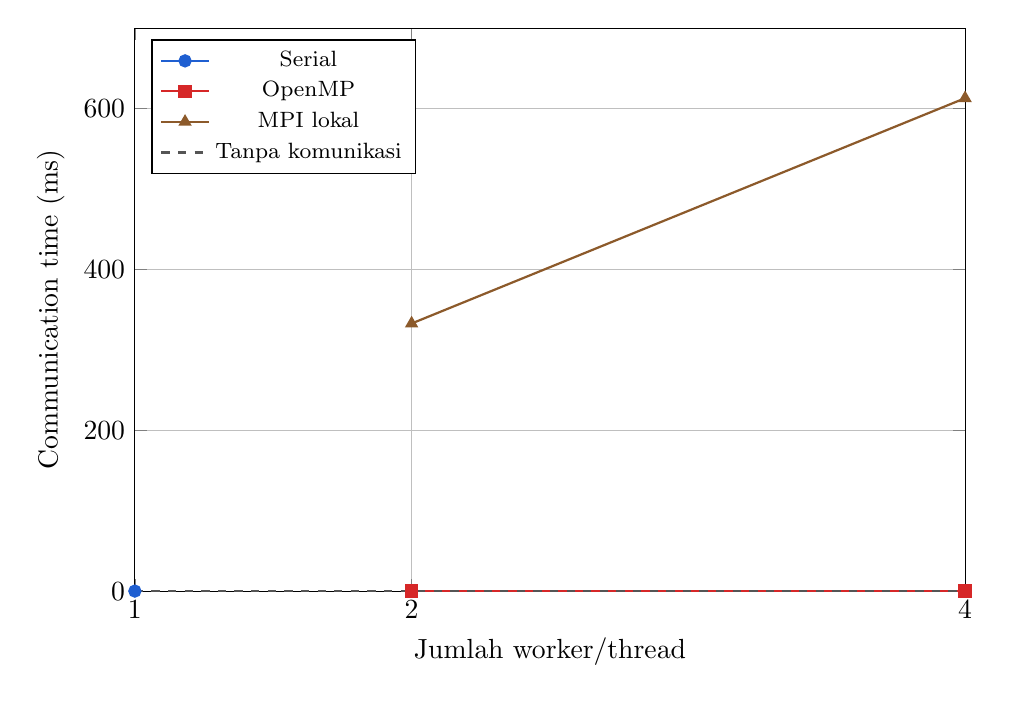
\begin{tikzpicture}
\begin{axis}[
    width=\columnwidth,
    height=0.72\columnwidth,
    xlabel={Jumlah worker/thread},
    ylabel={Communication time (ms)},
    xmin=1,
    xmax=4,
    ymin=0,
    ymax=700,
    xtick={1,2,4},
    ytick={0,200,400,600},
    grid=major,
    legend style={
      font=\footnotesize,
      at={(0.02,0.98)},
      anchor=north west,
      draw=black,
      fill=white
    }
]
\addplot+[serialblue, mark=*, thick, mark options={fill=serialblue}] coordinates {(1,0.0)};
\addlegendentry{Serial}
\addplot+[openmpred, mark=square*, thick, mark options={fill=openmpred}] coordinates {(2,0.0) (4,0.0)};
\addlegendentry{OpenMP}
\addplot+[mpibrown, mark=triangle*, thick, mark options={fill=mpibrown}] coordinates {(2,332.7728) (4,613.0017)};
\addlegendentry{MPI lokal}
\addplot+[baselinegray, dashed, thick, mark=none] coordinates {(1,0.0) (4,0.0)};
\addlegendentry{Tanpa komunikasi}
\end{axis}
\end{tikzpicture}
\caption{Communication time pada serial, OpenMP, dan MPI lokal.}
\label{fig:commplot}
\end{figure}

Communication time pada MPI lokal tercatat 332.7728 ms untuk 2 proses dan 613.0017 ms untuk 4 proses. Nilai ini besar dibandingkan waktu serial. Pada implementasi ini, communication time merupakan akumulasi waktu komunikasi dan probing antar-rank. Karena dikumpulkan dari beberapa proses dan beberapa operasi, nilainya dapat tampak lebih besar daripada satu pengukuran wall-clock tunggal.

Ada beberapa penyebab utama overhead MPI pada eksperimen ini. Pertama, setiap worker harus meminta task ke master dan menunggu balasan. Kedua, hasil recipe dikirim sebagai payload JSON sehingga ada biaya serialisasi dan parsing. Ketiga, master harus melakukan merge dan deduplikasi hasil. Keempat, memoization tidak dibagi secara global, sehingga reuse cache antar-rank tidak terjadi. Kelima, target \textit{Brick} dengan limit 50 bukan workload yang cukup berat untuk menutupi seluruh biaya tersebut.

\subsection{Implikasi}

Dari hasil ini, pendekatan OpenMP lebih cocok untuk eksperimen lokal dengan ukuran pencarian kecil sampai menengah. OpenMP memiliki overhead rendah dan dapat memanfaatkan beberapa core tanpa biaya message passing. MPI tetap penting karena menyediakan jalur ke multi-komputer, tetapi perlu workload yang lebih besar agar manfaatnya muncul. Untuk target yang memiliki ruang pencarian jauh lebih luas, split-depth yang tepat dan jumlah task yang cukup dapat membuat MPI lebih kompetitif.

\section{Kesimpulan}

Pencarian resep Little Alchemy 2 dapat dimodelkan dengan baik sebagai pencarian graf dependensi yang menghasilkan pohon resep. Implementasi serial menyediakan baseline yang stabil, OpenMP mempercepat sebagian proses BFS dengan overhead relatif kecil, sedangkan MPI memungkinkan pembagian kerja antar proses melalui model master-worker.

Berdasarkan eksperimen target \textit{Brick} limit 50, OpenMP 4 thread menghasilkan waktu terbaik, yaitu 86.4973 ms dengan speedup 1.072. OpenMP 2 thread juga lebih cepat dari serial dengan speedup 1.045. Namun, efisiensi keduanya belum tinggi karena workload relatif kecil dan masih ada bagian serial. MPI lokal 2 dan 4 proses lebih lambat dari serial, masing-masing dengan speedup 0.234 dan 0.171, karena overhead komunikasi dan koordinasi lebih dominan daripada komputasi pencarian.

Dengan demikian, untuk kasus benchmark ini, OpenMP adalah pendekatan paralel yang paling sesuai. MPI lebih cocok diuji pada target yang lebih kompleks, limit lebih besar, atau konfigurasi multi-komputer dengan task yang cukup banyak agar overhead komunikasi dapat teramortisasi.

\section{Saran}

Pengembangan berikutnya dapat diarahkan pada beberapa hal. Pertama, memilih target benchmark yang lebih berat agar perbedaan performa paralel lebih terlihat. Kedua, mengoptimalkan pembagian task MPI agar worker mendapat beban yang lebih seimbang. Ketiga, mengurangi ukuran payload hasil atau mengganti format komunikasi agar biaya serialisasi lebih kecil. Keempat, mengevaluasi hybrid MPI+OpenMP untuk memanfaatkan banyak komputer sekaligus menjaga overhead komunikasi tetap terkendali.

\begin{thebibliography}{00}

\bibitem{littlealchemyplay}
Recloak, ``Little Alchemy 2,'' Google Play. [Online]. Available: \url{https://play.google.com/store/apps/details?id=com.recloak.littlealchemy2}

\bibitem{littlealchemyhints}
Recloak, ``Little Alchemy 2 Official Hints and Cheats.'' [Online]. Available: \url{https://hints.littlealchemy2.com/}

\bibitem{openmp}
OpenMP Architecture Review Board, ``OpenMP,'' [Online]. Available: \url{https://www.openmp.org/}

\bibitem{mpiforum}
MPI Forum, ``MPI Forum,'' [Online]. Available: \url{https://www.mpi-forum.org/}

\bibitem{mpistandard}
MPI Forum, ``MPI: A Message-Passing Interface Standard Version 5.0,'' 2025. [Online]. Available: \url{https://www.mpi-forum.org/docs/mpi-5.0/mpi50-report/mpi50-report.htm}

\end{thebibliography}

\end{document}
